\documentclass{article}
\usepackage[T1]{fontenc}
\usepackage{lmodern}
\usepackage{graphicx}
\usepackage{amsmath,amssymb}
\usepackage[a4paper,margin=2cm]{geometry}
\usepackage[absolute,overlay]{textpos}
\setlength{\TPHorizModule}{1mm}
\setlength{\TPVertModule}{1mm}
\usepackage[indonesian]{babel}
\usepackage{hyperref}
\setlength{\emergencystretch}{2em}
% unit: Halaman 41

\begin{document}

% === Halaman 41 (llm) ===

\vspace{210.87mm}

Cek video GSM Sniffing: Voice Decryption 101 - Software Defined Radio Series \#11:\
\url{https://www.youtube.com/watch?v=krJKKjYdwgc}

\vspace{10mm}

GSM Sniffing: Voice Decryption 101 - Software Defined Radio Series \#11

% deskripsi: Screenshot video YouTube yang menampilkan perangkat lunak analisis sinyal radio (SDR) dan terminal command line untuk proses GSM sniffing.
% bbox normalisasi: [0.1500, 0.1500, 0.7500, 0.8600]
\begin{textblock*}{126.00mm}(31.50mm,44.55mm)
\noindent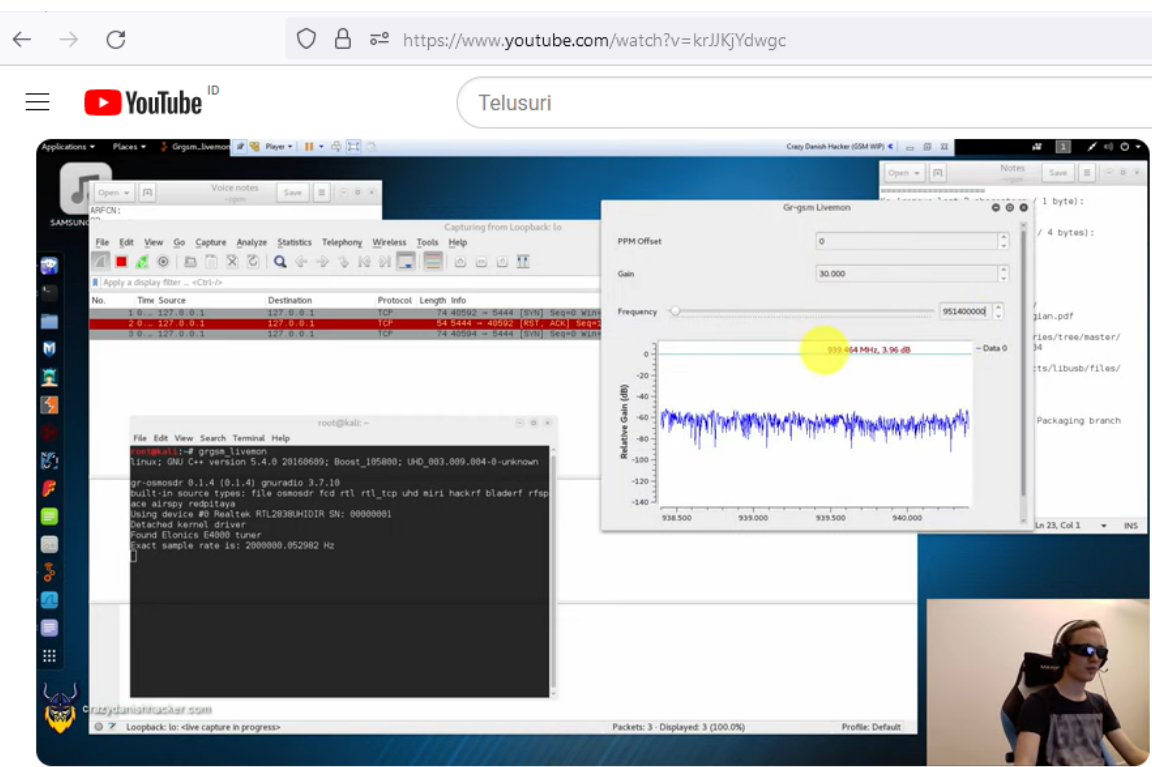
\includegraphics[width=126.00mm,height=210.87mm]{../../images/llm/page_041_img_01.png}%
\end{textblock*}

\end{document}
